%!TEX root=../../main.tex
\section{Frontend}
In diesem Kapitel geht es darum ein Konzept für das Frontend zu erstellen. Dabei müssen Faktoren wie beispielsweise unsere Zielgruppe, die Lehrerschaft beachtet werden. Im folgenden Kapitel werden die theoretischen Hintergründe des Konzeptes überlegt, danach werden erste Entwürfe mittels Mockups erstellt. 
\subsection{Theoretische Konzeption}
Da die Zielgruppe \enquote{Lehrer} nicht gleichaltrig ist, sondern die darin enthaltenen Menschen ein Alter von 25 bis 65 Jahren haben gibt es keine Literatur zur \enquote{perfekten Usability für Lehrpersonal}. Daher richten wir uns nach dem Buch \enquote{Don't Make Me Think: A Common Sense Approche to Web Usability} von Steve Krug und an dem Buch \enquote{101 UX Principles} von Will Grant. Um eine gute Usability für die Lehrer des TGMs zu gewährleisten werden wir den Prozess der Entwicklung streng in Kontakt zu Lehrern begleiten und das Produkt auch mit nicht Technik affinen Menschen testen.  
\subsection{Visuelle Konzeption}
\begin{figure}[H]
	\centering
	
\includegraphics[width=1\linewidth]{images/Mockup-Startseite}
	\caption[Mockup Login]{Das Mockup der Login Seite}
	\label{fig:mockupLogin}
\end{figure}
\begin{figure}[H]
	\centering
	
\includegraphics[width=1\linewidth]{images/Mockup-Startseite-eingeloggt}
	\caption[Mockup Startseite]{Das Mockup der Startseite, nachdem man sich eingeloggt hat}
	\label{fig:mockupStart}
\end{figure}
\begin{figure}[H]
	\centering
	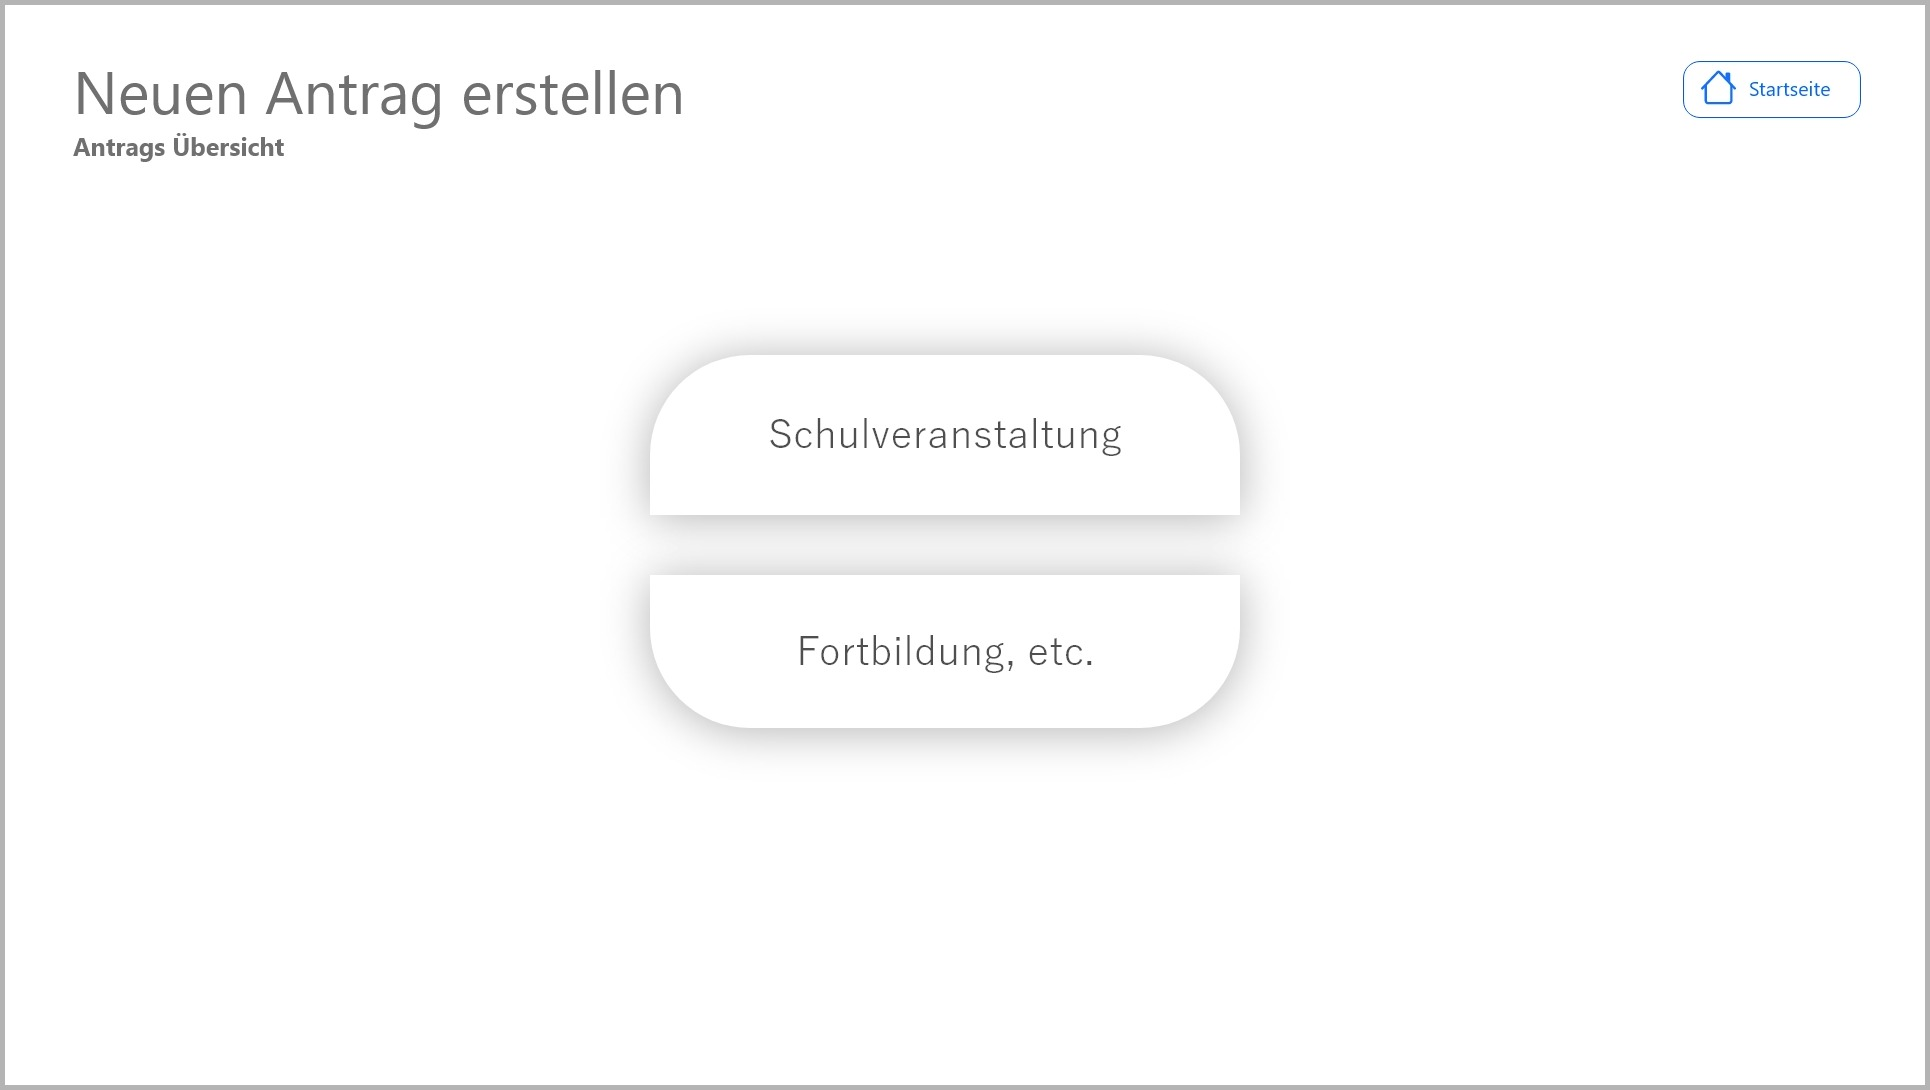
\includegraphics[width=1\linewidth]{images/Mockup-Neuer-Antrag}
	\caption[Mockup neuer Antrag]{Das Mockup der Seite, auf der man eine Antragsart auswählen kann}
	\label{fig:mockupNeu}
\end{figure}
\begin{figure}[H]
	\centering
	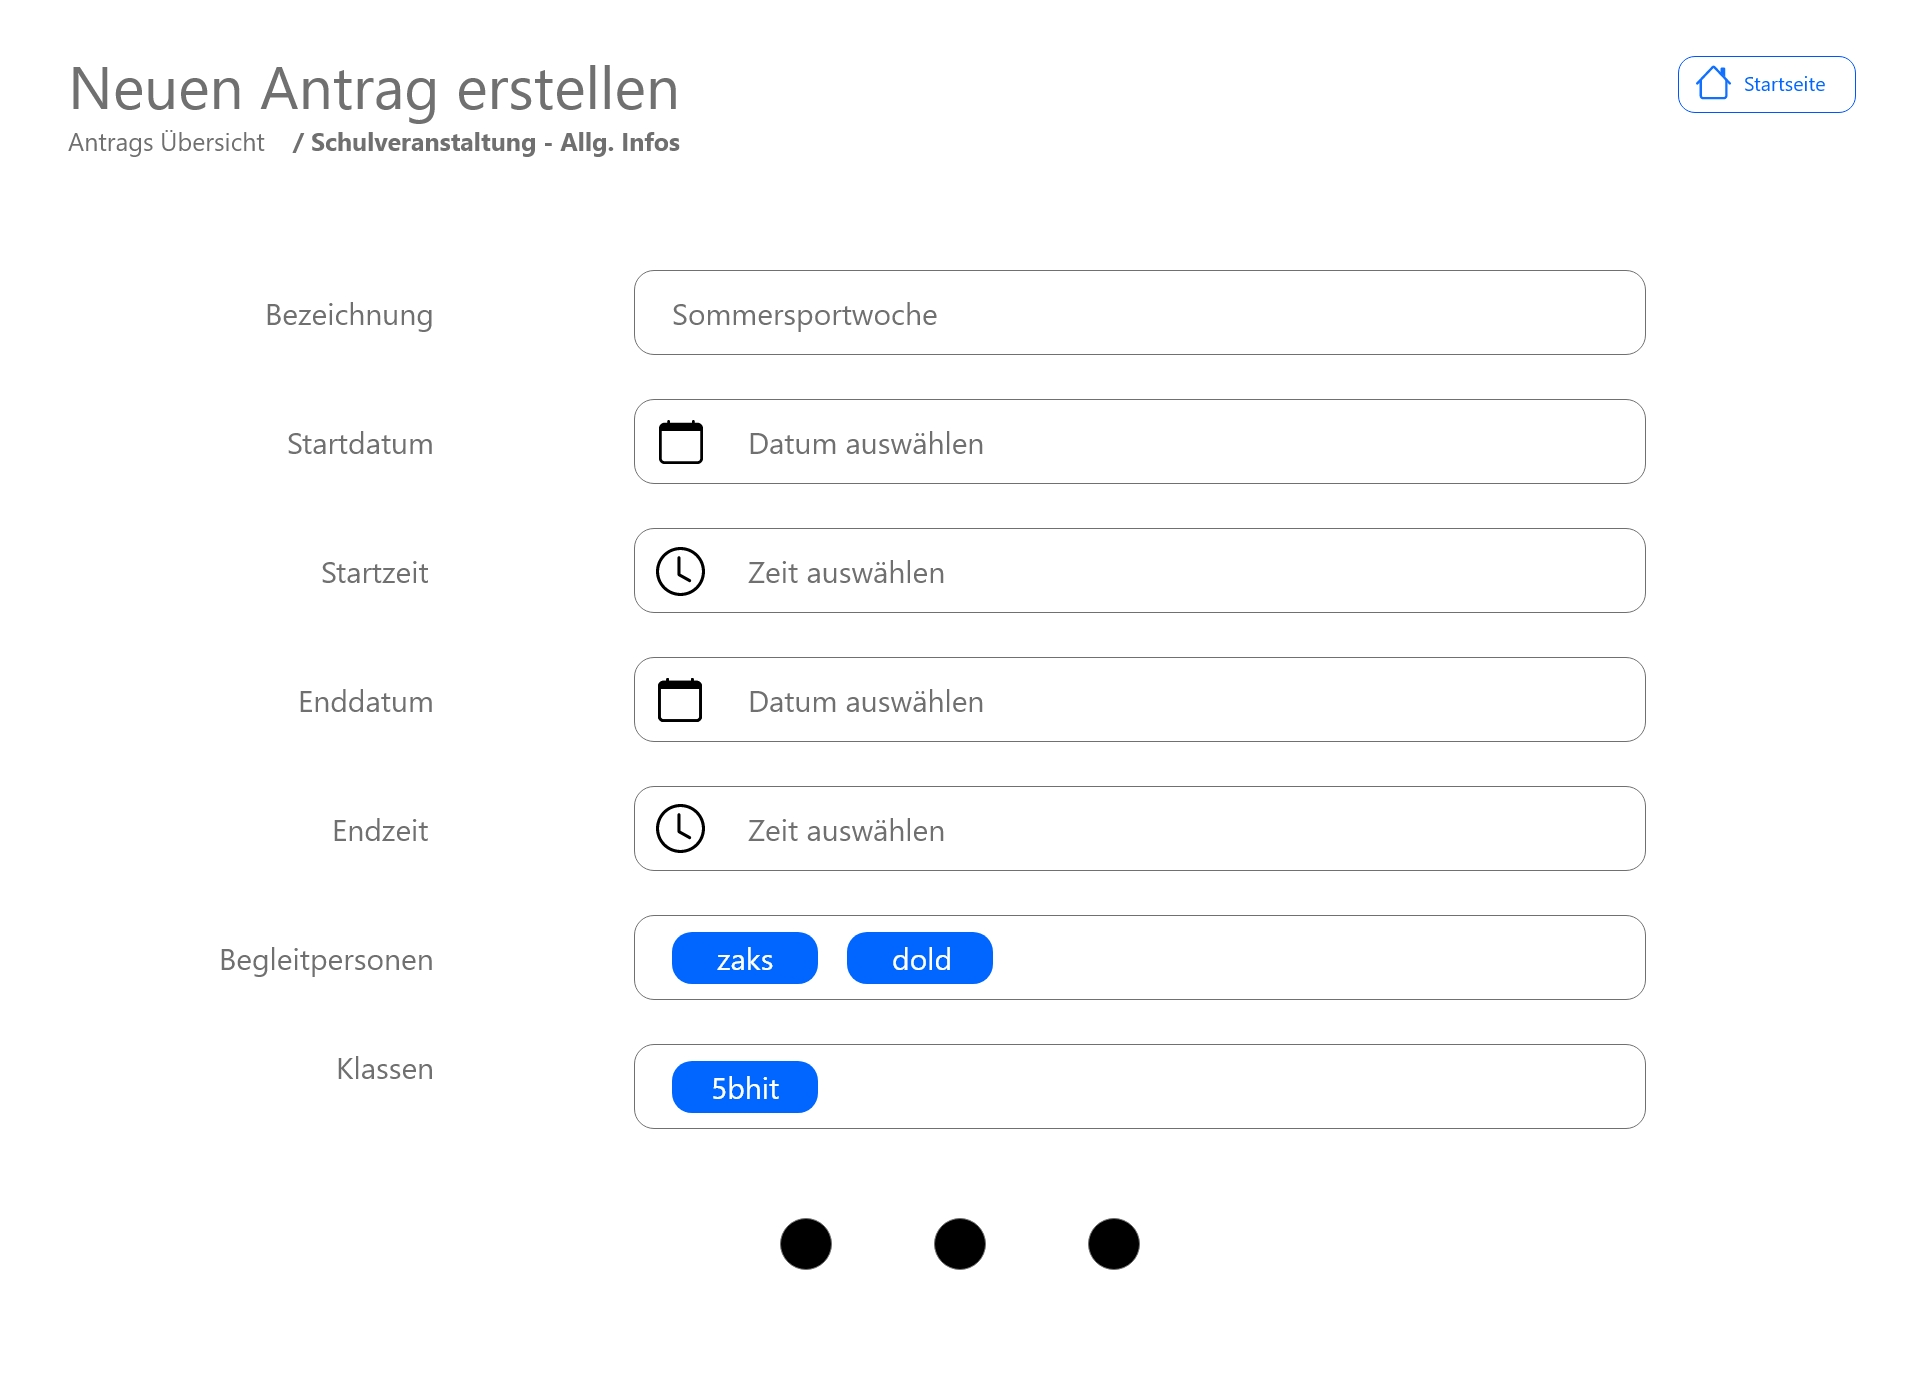
\includegraphics[width=1\linewidth]{images/Mockup-Antrag-erstellen}
	\caption[Mockup Antrag erstellen]{Das Mockup zum erstellen einer neuen Schulveranstaltung}
	\label{fig:mockupErstellen}
\end{figure}
\begin{figure}[H]
	\centering
	\includegraphics[width=1\linewidth]{images/Mockup-Alle-Anträge}
	\caption[Mockup Alle Anträge]{Das Mockup, welches alle Anträge einer gewissen Person veranschaulicht}
	\label{fig:mockupAlle}
\end{figure}
\begin{figure}[H]
	\centering
	\includegraphics[width=1\linewidth]{images/Mockup-Aktive-Anträge}
	\caption[Mokup aktive Anträge]{Das Mockup, welches alle aktiven Anträge einer gewissen Person veranschaulicht}
	\label{fig:mockupAktive}
\end{figure}
\begin{figure}[H]
	\centering
	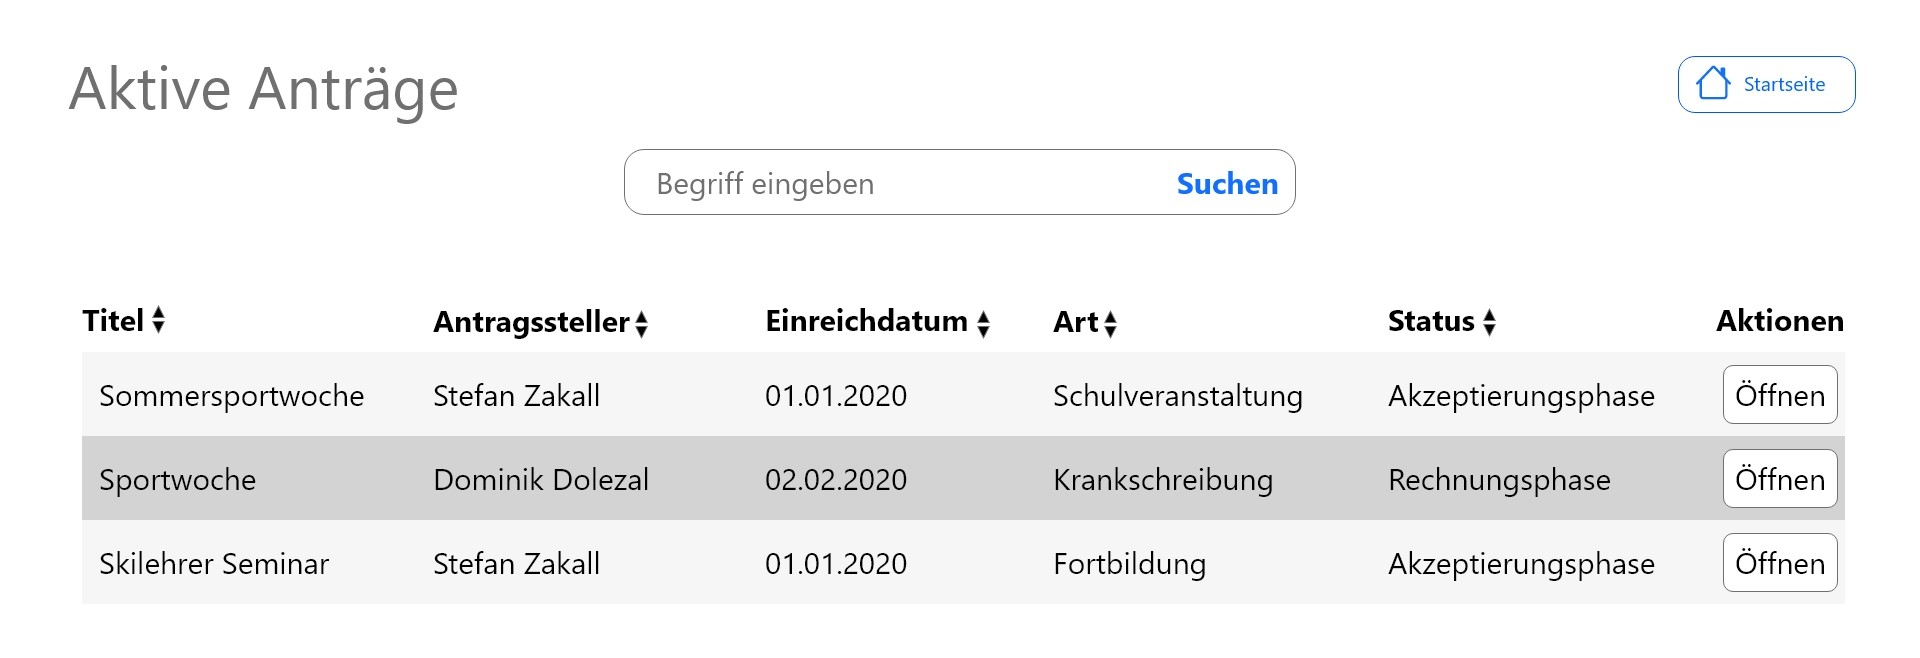
\includegraphics[width=1\linewidth]{images/Mockup-Admin}
	\caption[Mockup Adminansicht]{Das Mockup, der Admin Ansicht, zum akzeptieren und ablehnen von Anträgen}
	\label{fig:mockupAdmin}
\end{figure}
\begin{figure}[H]
	\centering
	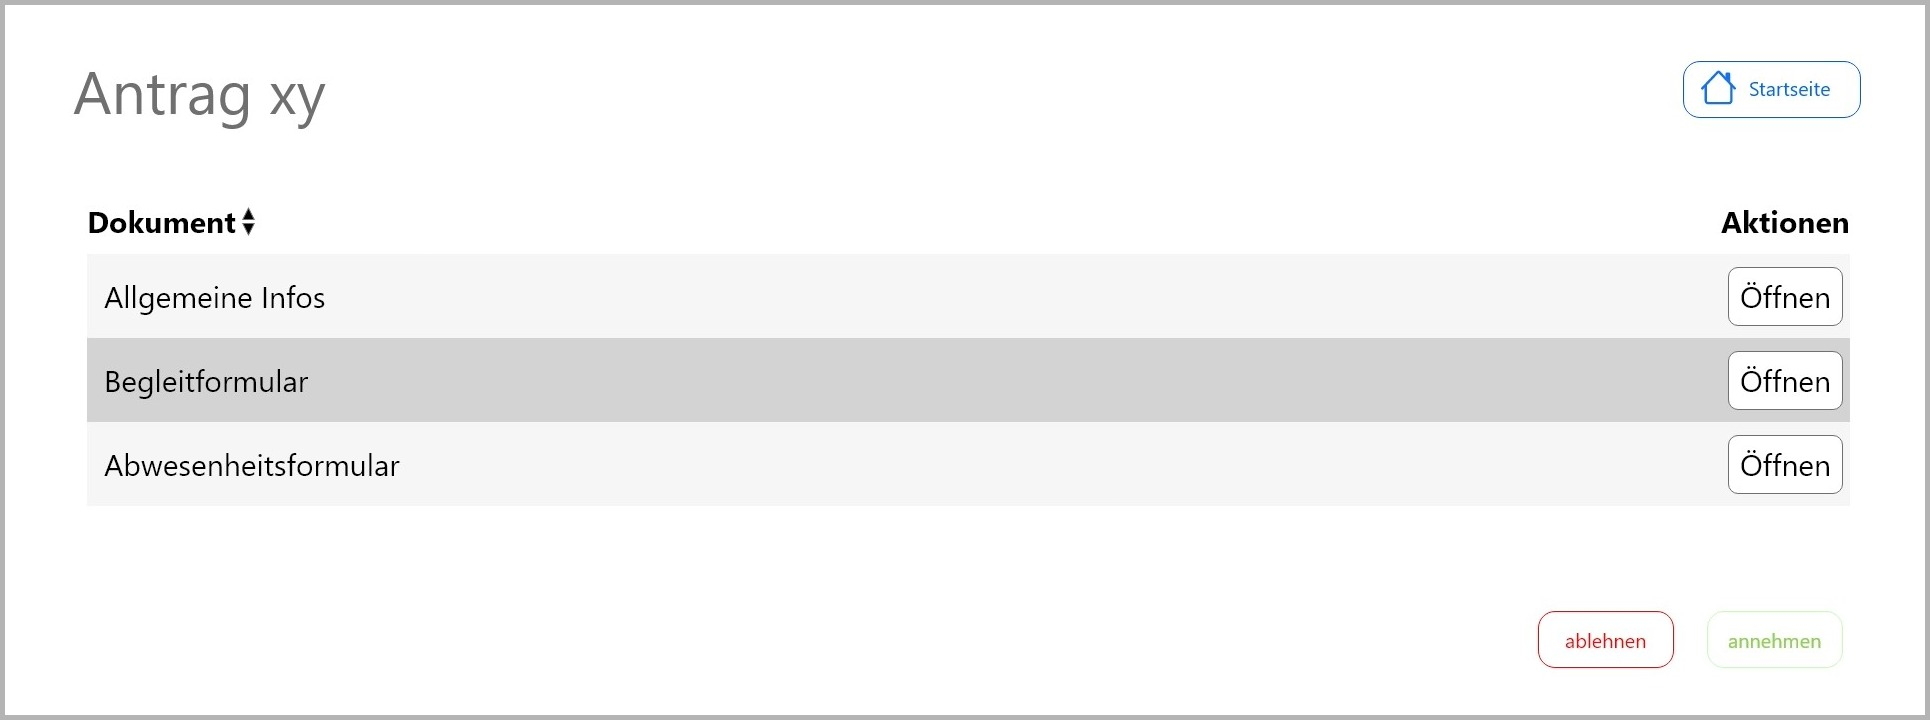
\includegraphics[width=1\linewidth]{images/Mockup-Antragsansicht}
	\caption[Mockup Antragsansicht]{Das Mockup, welches einen eingereichten Antrag veranschaulicht}
	\label{fig:mockupAntrag}
\end{figure}